% \documentclass[notes]{beamer}       % print frame + notes
\documentclass{beamer}   % only notes
%\documentclass{beamer}              % only frames
\usepackage{LlabsTheme}

\usepackage[utf8]{inputenc}
\usepackage[T1]{fontenc}
\usepackage[german, english]{babel}
\usepackage{amsmath,amssymb,amsthm}
\usepackage{makeidx}
\usepackage{graphicx}
\usepackage{xspace}
\usepackage{url}
\usepackage{comment}
\usepackage{caption}

\usepackage{memhfixc}
\usepackage{hyphenat}
\usepackage{xcolor}

\usepackage[square,numbers]{natbib}
\bibliographystyle{abbrvnat}

\usepackage{afterpage}
\usepackage{refcount}
\usepackage{graphicx}

\usepackage{tikz}
\usetikzlibrary{decorations.text}
\usepackage{xcolor}
\usetikzlibrary{shapes}

\usepackage{url}
\usepackage{comment}
\usepackage{xspace}
\usepackage{siunitx}
\sisetup{locale = US}
\DeclareSIUnit{\mph}{mph}
\setlength\abovecaptionskip{2pt}

\captionsetup[figure]{font=tiny,labelfont=tiny}

%% to propeerly type 1st 2nd 3rd, usw
\newcommand\nd{\textsuperscript{nd}\xspace}
\newcommand\rd{\textsuperscript{rd}\xspace}
\newcommand\st{\textsuperscript{st}\xspace}

\newcommand\nth{\textsuperscript{th}\xspace} %\th is taken already


%\usepackage{algorithm}
%\usepackage{algpseudocode}

% \usepackage{algorithm2e}
% \usepackage{algorithmic}

%\usepackage{ngerman}      % language set to new-german
\usepackage[utf8]{inputenc}   % coding of german special characters
\usepackage[absolute,overlay]{textpos}
\usepackage{array}
\usepackage{setspace}
\newcommand{\RNum}[1]{\uppercase\expandafter{\romannumeral #1\relax}}
\newcommand{\argmin}{\operatornamewithlimits{argmin}}
\newcommand{\argmax}{\operatornamewithlimits{argmax}}
\newcommand{\meth}[1]{\texttt{\textbf{#1}}}

\newcommand{\csharp}{C\#\xspace}

\newcommand{\HL}[1]{{\color{primarycolor} #1}}

\usepackage{tikz}

\usepackage{hyperref}
\usepackage{graphicx}

\newcommand{\coo}{\ensuremath{\mathrm{CO_2}}}

\newcounter{thmcount}
\newtheoremstyle{break}% name
{}%         Space above, empty = `usual value'
{}%         Space below
{}% Body font
{}%         Indent amount (empty = no indent, \parindent = para indent)
{\bfseries}% Thm head font
{}%        Punctuation after thm head
{\newline}% Space after thm head: \newline = linebreak
{}%         Thm head spec

\usepackage{etoolbox}


\theoremstyle{break}
\newtheorem{exmp}{Example}[thmcount]
\newtheorem{obs}{Observation}[thmcount]
\newtheorem{cor}{Corollary}[thmcount]
\newtheorem{defn}{Definition}[thmcount]
\newtheorem{lem}{Lemma}[thmcount]

\usepackage{adjustbox}

\newcommand{\outgoing}{\emph{outgoing}\xspace}
\newcommand{\return}{\emph{return}\xspace}

\newcommand{\punctual}{\emph{punctual}\xspace}
\newcommand{\tardy}{\emph{tardy}\xspace}

\renewcommand*{\thefootnote}{\fnsymbol{footnote}}



\title[OHC transportation considering bridge carrying capacity]{
\large
Optimal route selection for oversize and heavyweight
cargo transportation considering bridge carrying capacity
}

\author[Christian Wankm\"uller]{\small
Christian Wankm\"uller  \inst{1}
\and
Andreas Felsberger \inst{1}
\and
Christian Truden \inst{2}
}

\institute[LLabs]{\footnotesize
\inst{1} Department of Operations Management and Logistics, Alpen-Adria-Universit\"at Klagenfurt,
Klagenfurt, Austria
\and
\inst{2} Lakeside Labs GmbH, Klagenfurt, Austria
}
\date{\footnotesize
31\st European Conference on Operational Research,\\
University of West Attica, Athens, Greece,\\
July 11-16, 2021
}





%Customized settings to define the style of the presentation

%%%%COLORS %%%%
%defines the used color scheme
\colorsAAU

%\titlelogoAAU  %%AAU logo on title frame
% \titlelogoLLabsLUC  %%LLAbs and LUC logo on title frame
% \titlelogoLLabsEFRE
\titlelogoAAULLabsSweet

%%%%LOGOS ON FRAMES %%%
%defines which logos are displayed on the frame, if you want to change the logos
%for certain frames, just apply the command before the \begin{frame} command
%all following frames will have the defines appearance
% \logoAAU
% \logoLlabsLUC
\logoAAULlabs
%\logoNONE

%%%HEADLINE
% \headlineLEFT  %aligns the section overview in the headline LEFT
\headlineCENTER %spreads the  section overview in the headline evenly


%%%FOOTLINE
%Define the appearance of the footline
%\footlineNUMBER  % show number of current slide
\footlineNUMBERTOTAL  % also shows the total number of slides
%\footlineNONUMBER  %no number displays

%%%%AVAILABLE COLORS%%%
%the following colors are predefined for use with the \color{col} command
%-   primarycolor
%-  secondarycolor

\begin{document}


\begin{frame}[plain]{\titlepage}\end{frame}
  %
  %
  %
  %
  %
  %   \section{Introduction}
  %
  %
  %
  % \begin{frame}
  % \frametitle{Agenda}
  %   \begin{itemize}
  %     \item Introduction
  %     \item Mathematical Model
  %     \item Example of Application and Preliminary Results
  %     \item Next Steps and Conclusion
  %   \end{itemize}
  %  \tableofcontents
  %
  %  \end{frame}



  \section{Introduction}


 \begin{frame}
    \frametitle{Agenda}
\begin{itemize}
	\item Introduction
	\item Mathematical Model
	\item Example of Application
	\item Next Steps and Conclusion
    \end{itemize}
  \end{frame}

  \begin{frame}
    \frametitle{Motivation \RNum{1}}
    \begin{itemize}
      \item Since 2010 global freight continuously increases with forecasts predicting growth rates of 3.2\,\% until 2050 \cite{figura2020preferences, InternationalTransportForum}.
      \item Road transportation is expected to rise in importance due to its dominating role for domestic transportation (80\,\% of total volume of goods transported by trucks in the EU) \cite{Eurostat}.
      \item Increase in demand also holds true for the transportation of superheavy, bulky and extra-large goods, i.e. oversized and heavy weight cargoes (OHC) \cite{gavrilova2021analysis, Luo.2021}.
    \end{itemize}
  \end{frame}

  \begin{frame}
    \frametitle{Motivation \RNum{2}}
    \begin{itemize}
      \item OHC is typically associated with the transportation of industry goods (e.g. generators, turbines, construction equipment).
      \item Exceed maximum legal limits in terms of weight and/or size.
      \item May require complete road closures or detours and must be escorted by police and other law enforcement \cite{Luo.2021}.
    \end{itemize}

    \begin{figure}[!ht]
      \centering
      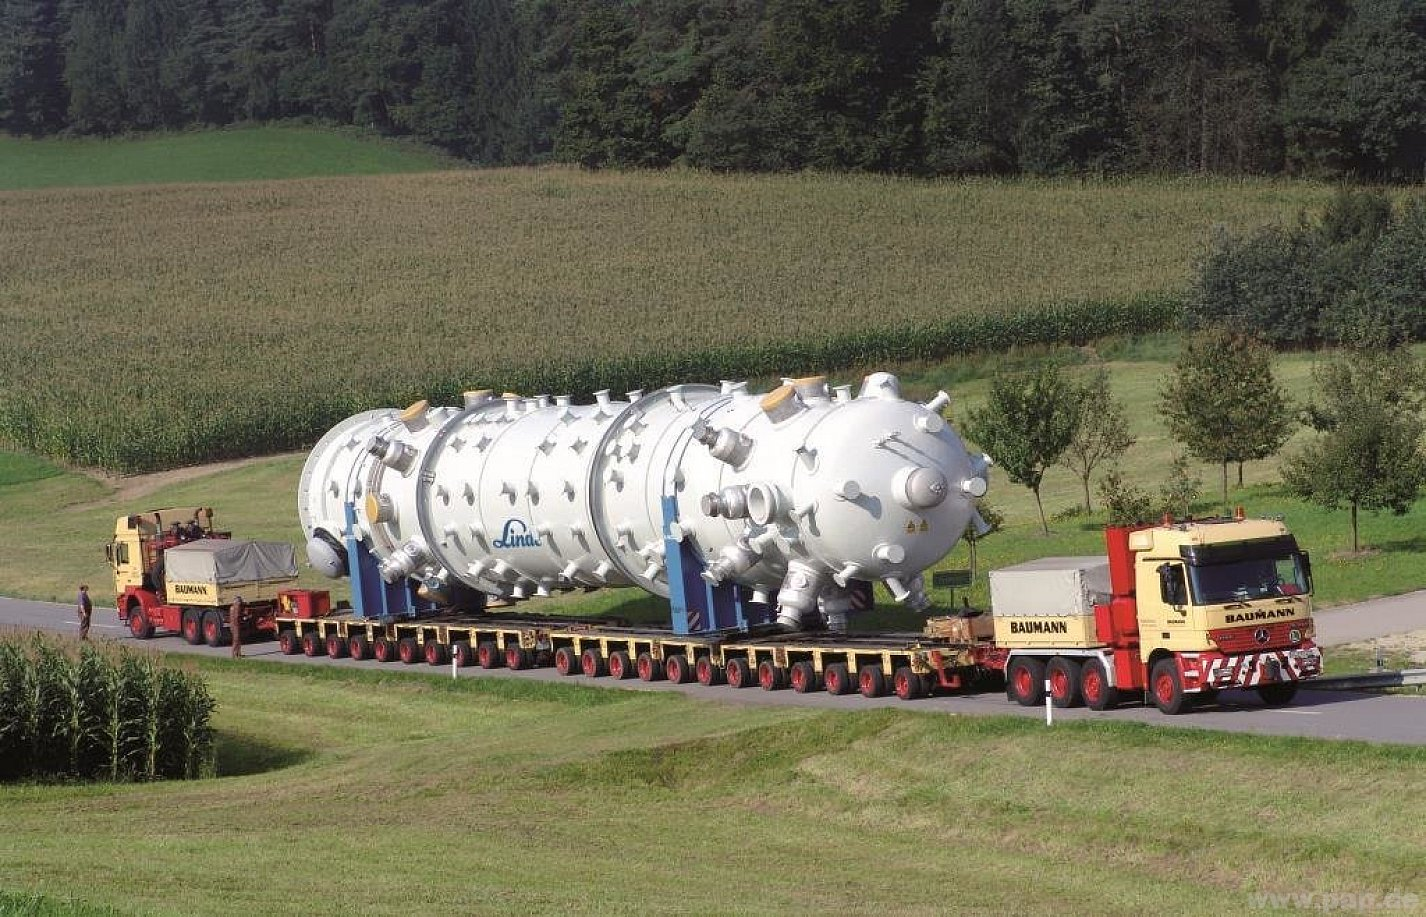
\includegraphics[width=0.5\textwidth]{../manuscript/figures/OHC.jpg}
      \caption{Typical OHC transport by truck.}
      \label{fig:higher level}
    \end{figure}

  \end{frame}

  \begin{frame}
    \frametitle{Planning of OHC transports  \RNum{1}}
    \begin{itemize}
      \item Technical, administrative and organizational criteria are subject of detailed analysis to reduce technical, economic, social and political risks \cite{Palsaitis.2012}.
      \item Granular planning is further dependent on national standards and legislations.
      \item Road turning radius, transportation corridor width and road-side obstacles, such as traffic lights or power lines \cite{PETRASKA.2018}.
      \item Maximum bridge carrying capacity, which must not be surpassed by the weight of total OHC transport when passing over.
    \end{itemize}
  \end{frame}

  \begin{frame}
    \frametitle{Planning of OHC transports  \RNum{2}}
    This is for two reasons:
    \begin{itemize}
      \item Overloading remarkably contributes to shorten service lifes of pavements and bridges
      \item Reduces bridge safety to levels that may fall below those set in the design standards \cite{fiorillo2018fragility}
    \end{itemize}
    \begin{figure}[!ht]
      \centering
      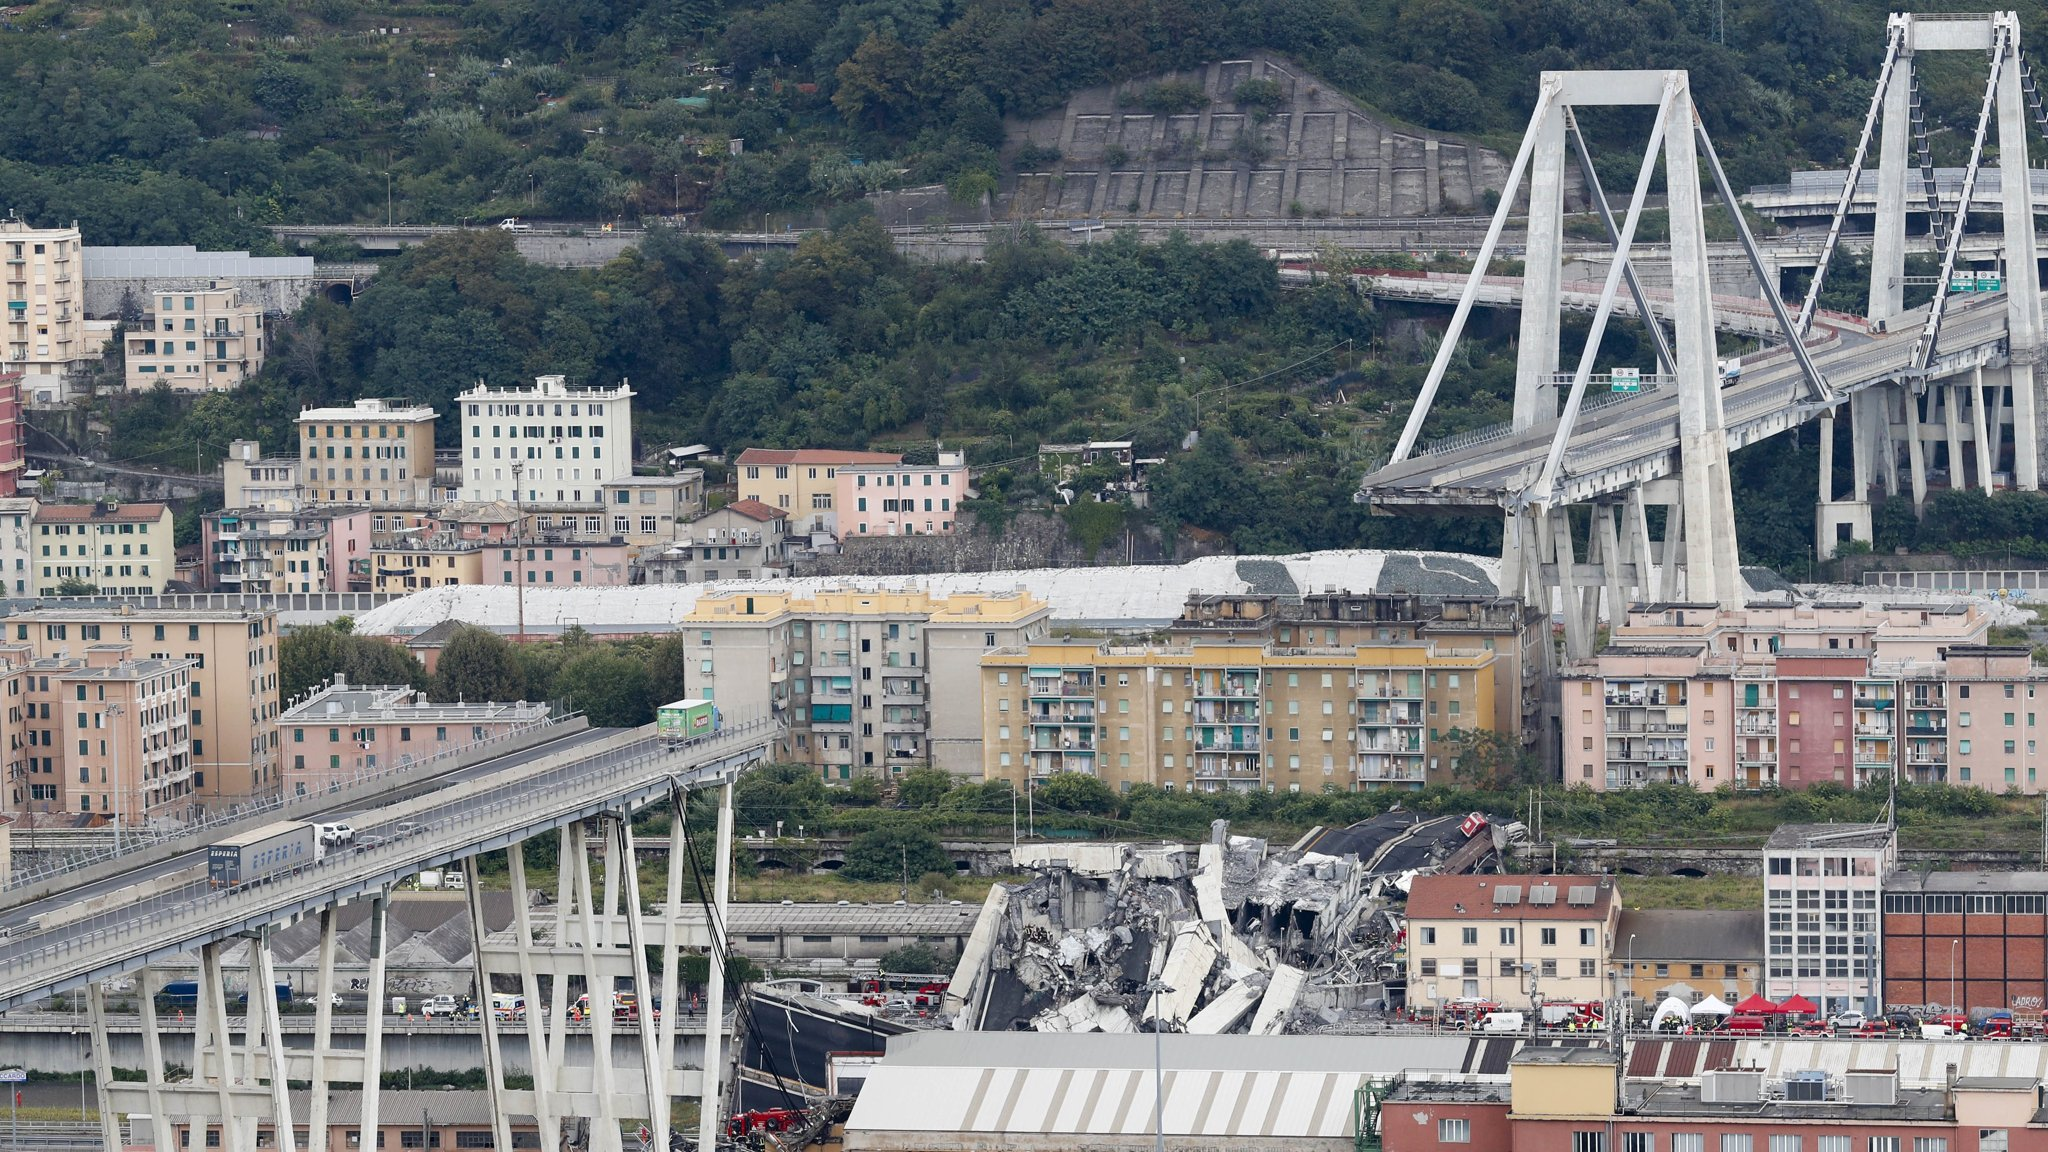
\includegraphics[width=0.5\textwidth]{../manuscript/figures/Collaps.jpg}
      \caption{Steps in OHC transport planning.}
      \label{fig:higher level}
    \end{figure}
  \end{frame}


  \begin{frame}
    \frametitle{Planning of OHC transports  \RNum{3}}
    \begin{figure}[!ht]
      \centering
      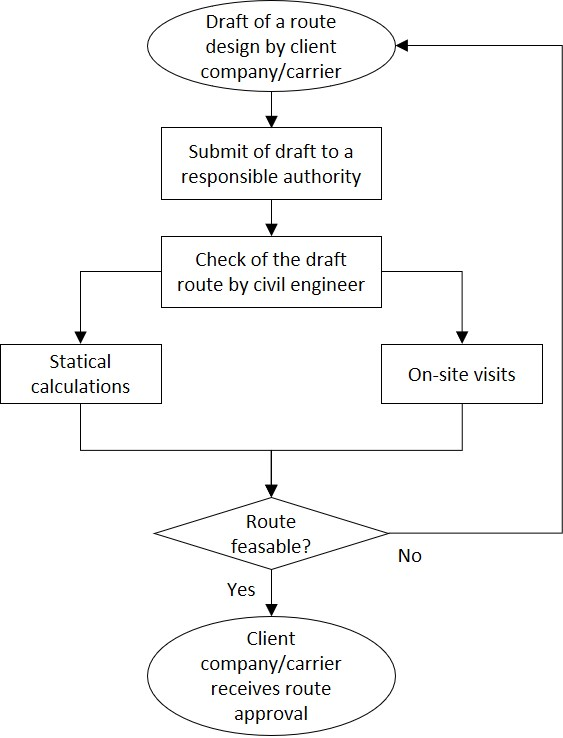
\includegraphics[width=0.4\textwidth]{../manuscript/figures/OHC Planning.jpg}
      \caption{Steps in OHC transport planning.}
      \label{fig:higher level}
    \end{figure}
  \end{frame}

  \begin{frame}
    \frametitle{Planning of OHC transports  \RNum{4} }
    \begin{itemize}
      \item Unexperienced users have problems in defining initial route design.
      \item Development of the initial route design is conducted primarily based on commercial GIS applications that are limited in terms of data accuracy.
      \item No information regarding road turning radius, maximum bridge carrying capacity etc. included.
      \item Costly and time-consuming process needs to be supported by adequate decision support.
      \item SWEET (Single Window for Exceptional Transport) has the objective to harmonize cross-border OHC transportation between Austria and Italy \cite{Sweet}.
    \end{itemize}
  \end{frame}




  \section[Mathematical Model]{Mathematical Model}
  \begin{frame}
    \frametitle{Road network representation}
    \begin{itemize}

      \item Classically,  the considered network $\mathcal{N}=(\mathcal{V},\mathcal{E})$ consists of
      \begin{itemize}
        \item \emph{Nodes} (vertices) $\mathcal{V}=\{1,\ldots, n\}$, which represent road  intersections as
        well as the start (end) points of the roads, and

        \item \emph{Links} (edges) $\mathcal{E} \subseteq \mathcal{L} \times \mathcal{L}$,
        correspond to the roads (road segements) connecting the vertices.
      \end{itemize}

      \item  Road links $e \in \mathcal{E}$ have a length $\ell(e)\in \mathbb{R}^{+}$ representing their road length.
      Further, they have a weights $c(e) \in C$ giving their national \emph{classification}.
      \item
      % Bridges have \emph{weight limits} (measured in metric tons) which are determined by civil engineers.
      Each road link $e \in \mathcal{E}$ contains a nonnegative number of bridges, where each has a weight limit.
      For each link $e$, we set a \emph{weight limit} $w(e) \in \mathbb{R}^{+}$ which is the
      minimum over all bridges on this link and the \emph{number of bridges} $b(e) \in \mathbb{N}^{0}$.

      \item Also  nodes $v \in \mathcal{V}$ can have weight limits.
    \end{itemize}

  \end{frame}



  \begin{frame}
    \frametitle{Transport requests}

    \begin{itemize}
      \item
      A \emph{transport request} $r=(o,d,w) \in \mathcal{V} \times \mathcal{V} \times \mathbb{R}^{+}$
      has an \emph{origin} $o$, a \emph{destination} $d$, a \emph{total weight} $w$.

      \item A transport $r$ can only pass through nodes $v \in \mathcal{V}$ with
      $w(r) \leq w(v)$ and traverse road links $e \in \mathcal{E}$ for which $w(r) \leq w(e)$ holds.

      \item We define the sub-network $\mathcal{N}_{\omega}$ that contains only the vertices and edges from $\mathcal{N}$ that have a weight limit larger than $\omega \in \mathbb{R}^{+}$.

      \item We set $\mathcal{N}=\mathcal{N}_{\omega=w(r)}$.
    \end{itemize}

  \end{frame}



  \begin{frame}
    \frametitle{Formulation}
    \begin{align}
      \min \quad &\sum_{(i,j)\in \mathcal{E}}  c_{ij} x_{ij} \label{obj} \\
      \text{s.t.}\quad &
      \sum_{(i,j)\in \delta^{+} (i)} x_{ji} - \sum_{(i,j)\in \delta^{-}(i)} x_{ij} =
      \begin{cases}
        1 \quad& \text{if}~ i=o, \\
        -1 \quad& \text{if}~ i=d \\
        0 \quad&\text{else}
      \end{cases}
      \qquad \forall i \in \mathcal{E}
      \\
      &  \sum_{(i,j)\in \delta^{+} (i)} x_ {ij} \leq 1     \qquad \forall i \in \mathcal{V}\\
      &  x_{ij} \in \{0,1\}   \qquad \forall (i,j) \in \mathcal{E}
    \end{align}
  \end{frame}


  \begin{frame}
    \frametitle{Objectives}
    We consider three different objectives, i.e., different assignment of $c_{ij}$.
    \begin{enumerate}
      \item \emph{Classic shortest path}, where $c_{ij}=\ell_{ij}$. \label{obj_short}
      \item \emph{Minimal number of surpassed briges}, where  $c_{ij}=b_{ij}$.  \label{obj_minBridge}
      \item \emph{Prefer high level roads}, where we assign an exponential weighting to the road classes (in ascending order of preference) $C$, $c_0=2^0,c_1=2^1, \ldots$.  \label{obj_highLevelRoad}
    \end{enumerate}
  \end{frame}


  \section[Example of Application] {Example of Application and Preliminary Results}
  \begin{frame}
    \frametitle{Example of Application}
    \begin{figure}[!ht]
      \centering
      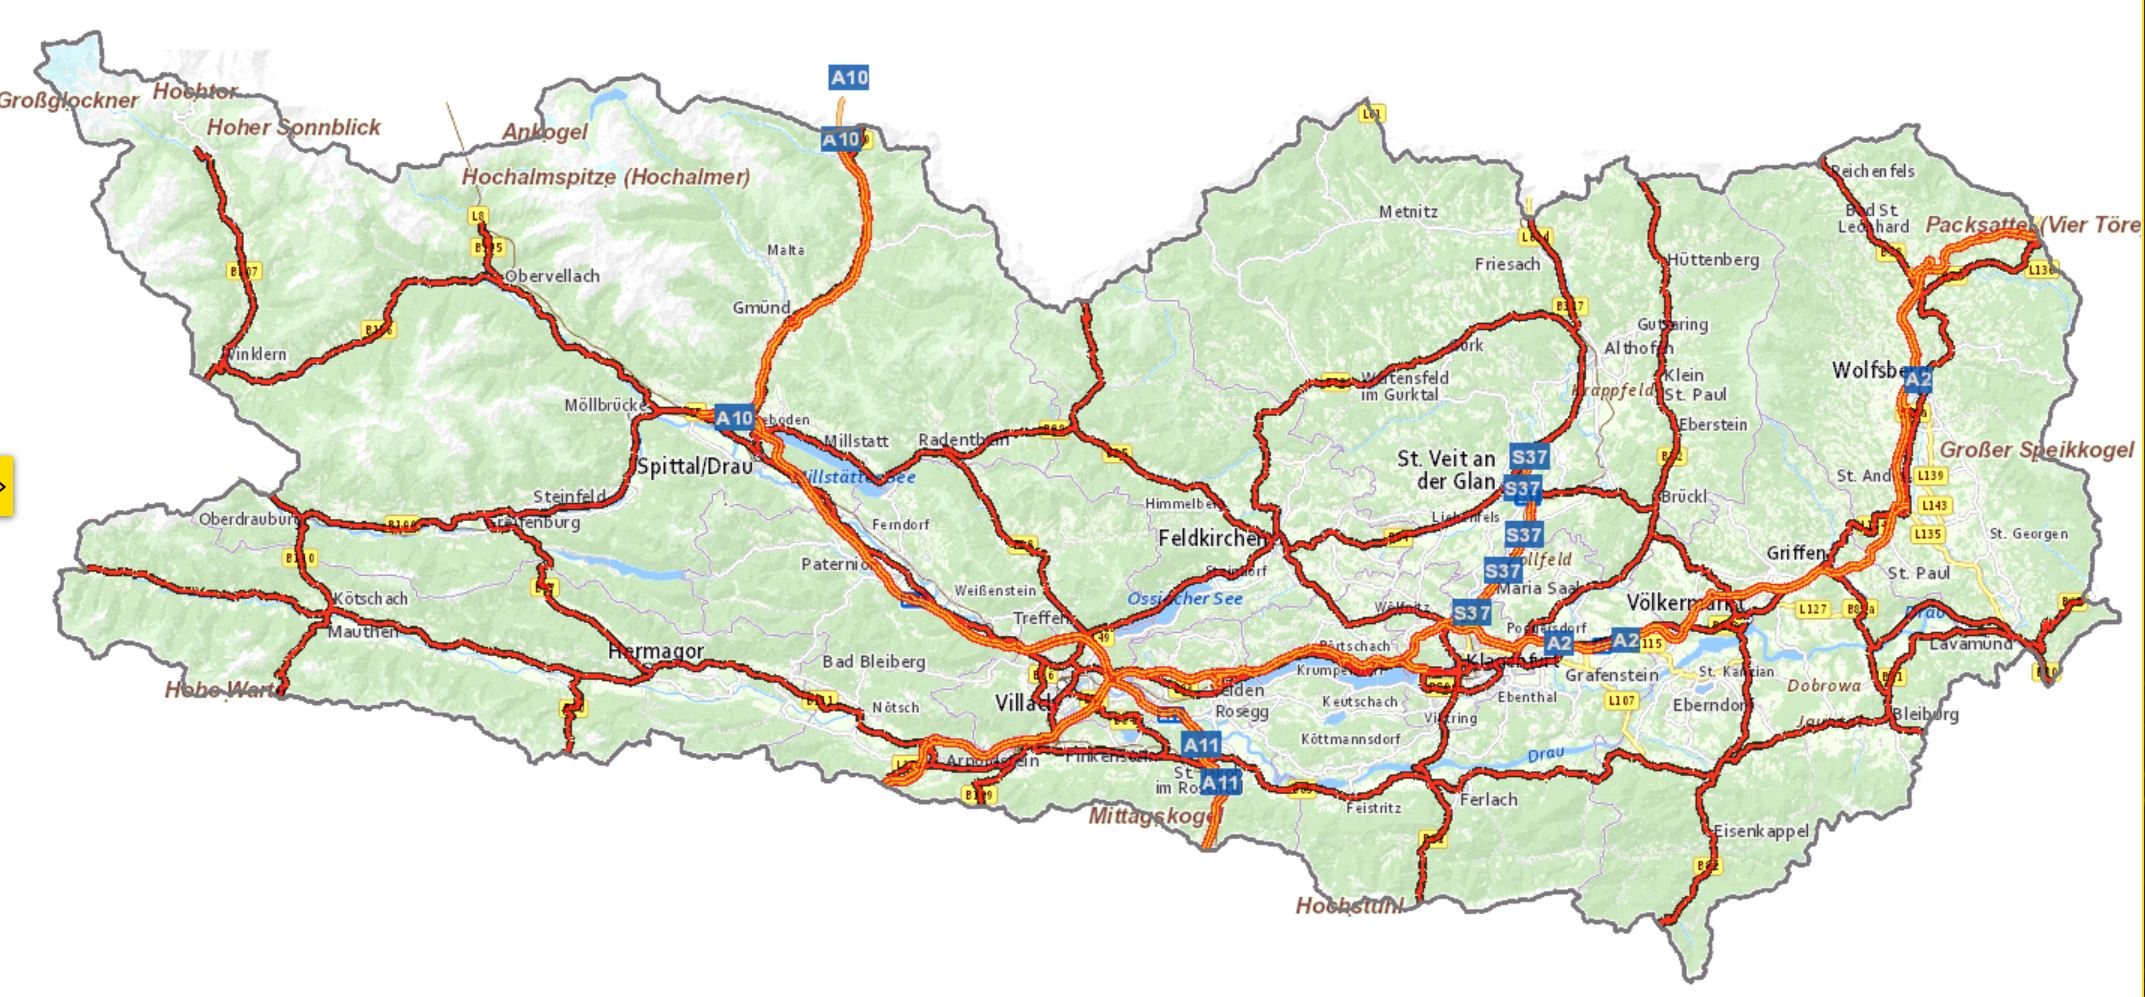
\includegraphics[width=1.0\textwidth]{../manuscript/figures/map.jpg}
      \caption{Overview of the higher level road network in Carinthia, Austria.}
      \label{fig:higher level}
    \end{figure}
  \end{frame}





  \begin{frame}
    \frametitle{Toy Example}
    \begin{figure}[!ht]
      \centering
      \scalebox{0.5}{
      % !TeX root =../main.tex
% !TeX spellcheck = en_US

% https://tex.stackexchange.com/questions/64252/tikz-midway-label-on-a-bended-line
% https://texample.net/tikz/examples/p2p-topology/

\begin{tikzpicture}[auto, thick]

  % Define Colors
  \definecolor{pinegreen}{cmyk}{0.92,0,0.59,0.25}
  \definecolor{royalblue}{cmyk}{1,0.50,0,0}
  \definecolor{lavander}{cmyk}{0,0.48,0,0}
  \definecolor{violet}{cmyk}{0.79,0.88,0,0}
  \definecolor{red}{cmyk}{0,0.95,0.90,0}
  \definecolor{yellow}{cmyk}{0,0.25,1,0}

  % Node styles
  \tikzstyle{cblue}=[circle, draw, thin,fill=cyan!20, scale=0.8]
  \tikzstyle{qgre}=[rectangle, draw, thin,fill=green!20, scale=0.8]

  \tikzstyle{A_path}=[ultra thick, red, opacity=0.8, font=\small]
  \tikzstyle{S_path}=[ultra thick, yellow, opacity=0.8, font=\small]
  \tikzstyle{B_path}=[ultra thick, royalblue, opacity=0.8, font=\small]
  \tikzstyle{L_path}=[ultra thick, pinegreen, opacity=0.8, font=\small]


  % Nodes
  % \node[cblue] (n_1_1) at (0,0) {1};
  % \node[cblue] (n_2_1) at (4,0) {2};
  \node[cblue] (n_6) at (8,0) {6};

  % \node[cblue] (n_1_2) at (0,4) {4};
  \node[cblue] (n_4) at (4,4) {4};
  \node[cblue] (n_5) at (8,4) {5};

  \node[cblue] (n_1) at (0,8) {1};
  \node[cblue] (n_2) at (4,8) {2};
  \node[cblue] (n_3) at (8,8) {3};




  %  A links

  \draw[A_path,postaction={decorate,decoration={text along path,text align=center,text={$d=3, ~w=10$},raise=-10pt}}](n_4)--  (n_5)  node [midway, above, sloped] {$[10t]$};
  \draw[A_path,postaction={decorate,decoration={text along path,text align=center,text={$d=3.7, ~w=10$},raise=-10pt}}] (n_6) to[bend left]   node [midway, above, sloped]  {$[10t]$} (n_5)  ;
  \draw[A_path, postaction={decorate,decoration={text along path,text align=center,text={$d=4, ~w=10$},raise=-10pt}}] (n_1) -- (n_4)  node [midway, above, sloped]  {$[10t]~[10t]$};


  % S links
  \draw[S_path, postaction={decorate,decoration={text along path,text align=center,text={$d=8, ~w=10$},raise=-10pt}}] (n_4) to node [midway, above, sloped] {$[10t]$} (n_6);

  %  L lines
  \draw[L_path, postaction={decorate,decoration={text along path,text align=center,text={$d=4, ~w=10$},raise=-10pt}}] (n_1) --  (n_2)  node [midway, above, sloped] (TextNode) {$[10t]$};

  \draw[L_path, postaction={decorate,decoration={text along path,text align=center,text={$d=5$},raise=-10pt}}] (n_2)--  (n_3)  node [midway, above, sloped] (TextNode) {};
  % \draw[L_path] (n_3) to[out=-20,in=-20]  (n_5)  node [midway, above, sloped] (TextNode) {$l=3, b=2$};
  \draw[L_path,postaction={decorate,decoration={text along path,text align=center,text={$d=3, ~w=10$},raise=-10pt}}] (n_3) to[bend left] node [midway, above, sloped]   {$[10t]$}    (n_5);

  \draw[L_path, postaction={decorate,decoration={text along path,text align=center,text={$d=4.5$},raise=-10pt}}] (n_5) to[bend left]  node [midway, above, sloped] {} (n_6);

  % B links
  % \draw[B_path] (n_6) to node [midway, above, sloped] {$7; 2$} (n_2_1);


  % Legends
  % \node[A_path, anchor=west] at (-3,8){\textsc{A:} $w=2^0$};
  % \node[S_path,anchor=west] at (-3, 7.5){\textsc{S:} $w=2^1$};
  % \node[L_path,anchor=west] at (-3, 7){\textsc{L:} $w=2^2$};
  % \node[B_path,anchor=west] at (-3, 6.5){\textsc{B:} $w=2^3$};

  \node[ anchor=west] at (0,2){Levels: {\color{red}\textsc{A}}, {\color{yellow}\textsc{S}},  {\color{royalblue}\textsc{B}},  {\color{pinegreen}\textsc{L}}  } ;


\end{tikzpicture}

      }
      % \caption{Toy Example 1.}
      % \label{fig_toy_example_1}
      % A simple toy example, see Figure \ref{fig_toy_example_1}, shall illustrate these definitions.
    \end{figure}
  \end{frame}


  \section[Next Steps and Conclusion] {Conclusion}

  \begin{frame}
    \frametitle{Next steps and Conclusion}
    \begin{itemize}
      \item Data on location (coordinates) and maximum carrying capacities of bridges on highway network is under process.
      \item Scenario development considering different truck load specifications.
	\item First step in providing decision-making support.
	\item Include also other restricting factors such as road turning radius.
    \end{itemize}

  \end{frame}



  %%%%%%%%%%%%%%%%%%%%%%%%%%%%%%%%%%%%%%%%%%%%%%%%%%%%%%%%%%%%%%%%



  %%%REFERENCES
  %if no references used, comment this section

  \appendix
  \begin{frame}[allowframebreaks]
    \frametitle{References}
    \vspace*{-1cm}
    \tiny
    \bibliographystyle{abbrvnat}
    \bibliography{../manuscript/bibliography}
  \end{frame}


  \begin{frame}[plain]{\titlepage}\end{frame}
    \end{document}
